\documentclass[]{article}

% Imported Packages
%------------------------------------------------------------------------------
\usepackage{amssymb}
\usepackage{amstext}
\usepackage{amsthm}
\usepackage{amsmath}
\usepackage{enumerate}
\usepackage{fancyhdr}
\usepackage[margin=1in]{geometry}
\usepackage{graphicx}
\usepackage{float}
%\usepackage{extarrows}
%\usepackage{setspace}
%\usepackage{xcolor}
\usepackage{color}
%------------------------------------------------------------------------------

% Header and Footer
%------------------------------------------------------------------------------
\pagestyle{plain}  
\renewcommand\headrulewidth{0.4pt}                                      
\renewcommand\footrulewidth{0.4pt}                                    
%------------------------------------------------------------------------------

% Title Details
%------------------------------------------------------------------------------
\title{Deliverable \#1 Template : Software Requirement Specification (SRS)}
\author{SE 3A04: Software Design II -- Large System Design}
\date{}
                            

%------------------------------------------------------------------------------

% Document
%------------------------------------------------------------------------------
\begin{document}
\setlength\parindent{0pt} 
\setlength{\parskip}{\baselineskip}

\maketitle	
\noindent{\bf Tutorial Number:} T0x\\
{\bf Group Number:} G07 \\
{\bf Group Members:} 
\begin{itemize}
	\item Farid Bastoros 
	\item 
	\item 
	\item
	\item  
\end{itemize}

\section*{IMPORTANT NOTES}
\begin{itemize}
	\item Be sure to include all sections of the template in your document regardless whether you have something to write for each or not
	\begin{itemize}
		\item If you do not have anything to write in a section, indicate this by the \emph{N/A}, \emph{void}, \emph{none}, etc.
	\end{itemize}
	\item Uniquely number each of your requirements for easy identification and cross-referencing
	\item Highlight terms that are defined in Section~1.3 (\textbf{Definitions, Acronyms, and Abbreviations}) with \textbf{bold}, \emph{italic} or \underline{underline}
	\item For Deliverable 1, please highlight, in some fashion, all (you may have more than one) creative and innovative features. Your creative and innovative features will generally be described in Section~2.2 (\textbf{Product Functions}), but it will depend on the type of creative or innovative features you are including.
\end{itemize}

\newpage
\section{Introduction}
\label{sec:introduction}
% Begin Section

\begin{itemize}
	\item Provide an overview of the document/SRS.
\end{itemize}


\subsection{Purpose}
\label{sub:purpose}
% Begin SubSection
\begin{itemize}
	\item Specify the purpose of the SRS.
	\item Specify the intended audience for the SRS.
\end{itemize}
% End SubSection

\subsection{Scope}
\label{sub:scope}
% Begin SubSection
\begin{itemize}
	\item Identify the software product(s) to be produced, and name each (e.g., Host DBMS, Report Generator, etc.)
	\item Explain what the software product(s) will do (and, if necessary, also state what they will not do).
	\item Describe the application of the software being specified, including relevant benefits, objectives, and goals.
%	\item Be consistent with similar statements in higher-level specifications (e.g., the system requirements specification), if they exist
\end{itemize}

\noindent
Mushroom.id, the mushroom identification application will allow users to identify mushrooms based on data collected in the field while foraging. The application is expected to use three
independent sources of identification called "experts". The experts are not intended to be real individuals, but rather software components that will provide identification based on user provided data. 

\vspace{0.5cm}
\noindent
The three experts are expected to be:

\begin{itemize}
	\item Macro Photo Expert: This expert will use a photo of the mushroom taken using a camera to identify the mushroom. THe user will be required to take a photo of the mushroom and upload it to be the application. The expert based on a CNN (Convolutional Neural Network) will identify the mushroom along with a probability.
	\item Micro Photo Expert: This expert will use a photo of the mushroom taken using a microscope to identify the mushroom. The user will be required to take a photo of the mushroom under a microscope and upload it to the application. The expert based on a CNN (Convolutional Neural Network) will identify the mushroom along with a probability.
	\item Text Description Expert: This expert will use textual descriptions of the mushroom, the location of the mushroom and other relevant information to identify the mushroom. The user will be required to input the textual information into the application. The expert based on a NLP (Natural Language Processing) model will identify the mushroom along with a probability.
\end{itemize}

Mushroom.id is not expected to provide any guarantees regarding the classification of the mushrooms, only a confidence percentage with a classification ranging from 0-100\%
Each expert module is expected to output a confidence probability ranging from 0.0 to 1.0 and a forum component will use each output and confidence probability to make the final decision.

If the user chooses to accept the mushroom identification outputted by the application, the application will also provide the user with a list of similar mushrooms and recipes that can be prepared using the identified mushroom.

To use the application the user is required to create an account so that the application can create a profile for the user to store their previous identifications and preferences. The user will also be able to access the application without creating an account, but the application will not store any of the user's data.
% End SubSection

\subsection{Definitions, Acronyms, and Abbreviations}
\label{sub:definitions_acronyms_and_abbreviations}
% Begin SubSection
\begin{itemize}
	\item Provide the definitions of all terms, acronyms, and abbreviations required to properly interpret the SRS.
	\item This should be in alphabetical order.
\end{itemize}
% End SubSection

\subsection{References}
\label{sub:references}
% Begin SubSection
\begin{itemize}
	\item Provide a complete list of all documents referenced elsewhere in the SRS.
	\item Identify each document by title, report number (if applicable), date, and publishing organization.
	\item Specify the sources from which the references can be obtained.
	\item Order this list in some sensible manner (alphabetical by author, or something else that makes more sense).
\end{itemize}
% End SubSection

\subsection{Overview}
\label{sub:overview}
% Begin SubSection

Section 2 will be discussing the overall product description and describe the general factors that affect the product. This will include product perspective and functions, user characteristics, assumptions and dependencies, and apportioning of requirements. Section 3 includes a Use Case Diagram for the scenario of identifying a mushroom in the wild. Section 4 highlights the function requirements and specifies all the uses cases by their Business Events. Section 5 will then move on to Non-Functional requirements, discussing look and feel, usability and humanity, performance, security, and cultural and political requirements. Finally, section A contains a division of labour.

% End SubSection

% End Section

\section{Overall Product Description}
\label{sec:overall_description}
% Begin Section

\begin{itemize}
	\item This section should describe the general factors that affect the product and its requirements. 
	\item It does not state specific requirements.
	\item It provides a \emph{background} for those requirements and makes them easier to understand.
\end{itemize}


\subsection{Product Perspective}
\label{sub:product_perspective}
% Begin SubSection
[Name] is a mobile mushroom identification app that allows users to submit a text description, macro photo, or micro photo of a mushroom and get detailed information on it. It will function similarly to Google Lens which lets users identify objects with their camera, but it will be specifically tailored to fungi allowing for more accuracy. The product will use state of the art machine learning-based services to determine the species. Location data will be used to narrow down the results, allowing for more accuracy. Users will have a profile where they can save their mushrooms, similar to a Pokedex.\\

The system will interact with Plant.id's identification api and [SYSTEM FOR ANALYZING TEXT DATA] in order to determine the specific fungi and if it is edible. It will be clarified to the user that they are only to consume the mushrooms at their own risk. If the mushroom is determined to be edible, the product will recommend recipes the user can cook using said mushroom. \\

\begin{figure}[h!]
    \centering
    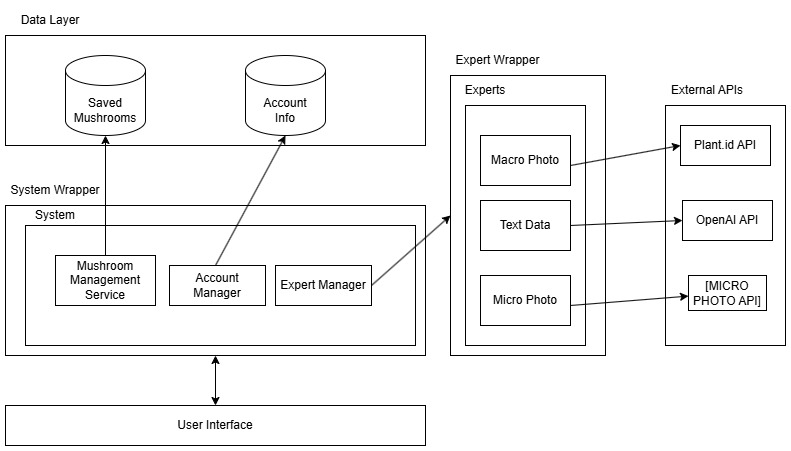
\includegraphics[width=0.9\textwidth]{BlockDiagram.jpg}
    \caption{System Diagram.}
    \label{fig:example}
\end{figure}
% End SubSection

\subsection{Product Functions}
\label{sub:product_functions}
% Begin SubSection
\begin{itemize}
	\item Provide a \emph{summary} of the major functions that the software will perform.
	\begin{itemize}
		\item \textbf{Example}: An SRS for an accounting program may use this part to address customer account maintenance, customer statement, and invoice preparation without mentioning the vast amount of detail that each of those functions requires.
	\end{itemize}
	\item Functions should be organized in a way that makes the list of functions understandable to the customer or to anyone else reading the document for the first time 
	\item Present the functions in a list format - each item should be one function, with a brief description of it
	\item Textual or graphical methods can be used to show the different functions and their relationships
	\begin{itemize}
		\item Such a diagram is not intended to show a design of a product, but simply shows the logical relationships among variables
	\end{itemize} 
\end{itemize}
% End SubSection

\begin{table}[H]
	\centering
	
	\label{tab:product_functions}
	\begin{tabular}{|c|p{10cm}|}
		\hline
		\textbf{Modules} & \textbf{Functions} \\
		\hline
		\hline
		\textbf{Decision Forum} & \begin{itemize}
			\item Mushroom Identification: The decision forum shall poll experts based on inputs provided to attempt to identify a mushroom.
			\item User Input: The decision forum shall accept three user inputs - a macro photo, a micro photo, and a text description and validate the inputs.
			\item Voting: The decision forum shall poll the experts and output a final decision based on the expert's outputs and confidence probabilities.
		\end{itemize} \\
		\hline
		\textbf{Account Manager} & \begin{itemize}
			\item Account creation: The account manager shall allow users to register and create an account.
			\item Account deletion: The account manager shall allow users to delete their account.
			\item Account modification: The account manager shall allow users to modify their account.
			\item Account login/logout: The account manager shall allow users to login and logout of their account.
		\end{itemize} \\
		\hline
		\textbf{Recipe Recommender} & \begin{itemize}
			\item Recipe Identification: The recipe recommender shall recommend a list of recipes based on the identified mushroom.
			\item Recipe Filtering: The recipe recommender shall allow users to filter the list of recipes based on dietary restrictions.
			\item Recipe Favoriting: The recipe recommender shall allow users to favorite recipes.
		\end{itemize} \\
		\hline
	\end{tabular}
	\caption{Product Functions}
\end{table}

\subsection{User Characteristics}
\label{sub:user_characteristics}
% Begin SubSection
General characteristics of the intended users of the product:
\begin{enumerate}
	\item Education Level: Basic Literacy required
	\begin{itemize}
		\item Users with the ability to read, write, and comprehend simple instructions should face no problems using the app.
	\end{itemize}
	\item Experience: No prior experience required
	\begin{itemize}
		\item First-time users should be able to navigate without difficulty, as the app is assumed to be user-friendly.
	\end{itemize}
	\item Technical Expertise: Familiarity with touchscreen devices
	\begin{itemize}
		\item Users with basic knowledge of touchscreen interactions, such as swiping, tapping, and typing, should have no issues using the app.
	\end{itemize}
\end{enumerate}
% End SubSection

\subsection{Constraints}
\label{sub:constraints}
% Begin SubSection
\begin{itemize}
	\item Provide a general description of any constraints that will limit the developer's options
\end{itemize}
% End SubSection

\subsection{Assumptions and Dependencies}
\label{sub:assumptions_and_dependencies}
% Begin SubSection
Assumptions made while interpreting what the software being developed aims to achieve.
\begin{enumerate}
	\item The function of identifying a mushroom is different from discovering the different types of mushrooms.
	\item \textbf{\textcolor{red}{Innovative feature 1:}} The user can collect mushrooms. When they identify one, it's saved to their account as a collected mushroom.
	\item \textbf{\textcolor{red}{Innovative feature 2:}} After the user has found an edible mushroom, they can find recipes for it.
	\item Assume "Identify Mushroom using photo" implies displaying the camera app to take a picture.
	\item The app will only be used in Canada.
\end{enumerate}

Other assumptions that, if it fails to hold, could require a change to the requirements:
\begin{enumerate}
	\item The product shall have uninterrupted access to an internet connection.
    \item Assume that users have granted all necessary permissions for the app to function properly.
    \item Assume that third-party libraries and dependencies remain compatible with future updates.
    \item Assume that APIs remain compatible with future updates.
\end{enumerate}
% End SubSection

\subsection{Apportioning of Requirements}
\label{sub:apportioning_of_requirements}
% Begin SubSection
\begin{itemize}
	\item \textbf{Varying Language Options:} The initial version of the app only supports English; however, in the future, additional language options will be implemented to create a more inclusive environment for a broader user base.
	\item \textbf{Offline Usage:} The initial release of the application will require an internet connection to identify mushrooms. Future versions may include an offline identification feature, allowing users to access identification tools without being connected to an internet network.
	\item \textbf{VR/AR for Mushroom Identification:} In the initial release, the app will rely on macro and micro photos for identification, with users being presented with a new screen of information regarding the identified mushroom. A future update may include augmented reality (AR) functionality that overlays information about mushrooms directly onto the camera’s view in real time.
	\item \textbf{Competitive Gameplay:} While the initial version focuses on individual mushroom identification, future updates may include competitive gaming features to create a more engaging experience for users. This could be implemented with a leaderboard ranking users based on the number of mushrooms identified or rare mushroom discoveries.
\end{itemize}
% End SubSection

% End Section
\section{Use Case Diagram}
\label{sec:use_case_diagram}
% Begin Section
\begin{itemize}
	\item Provide the use case diagram for the system being developed.
	\item You do not need to provide the textual description of any of the use cases here (these will be specified under "Highlights of Functional Requirements").
%	\item Provide \emph{one} use case diagram for the most important Business Event.
%	\item The text of all use cases will be specified under "Highlights of Functional Requirements"
\end{itemize}
%In this section, select the most important Business Event that your system responds to and give its use case diagram.  Only one use case diagram is needed.  Give a brief textual description of the use case without repeating what is in the scenarios of the corresponding Business Event.

%
%
%
%This section should provide a use case diagram for your application. 
%\begin{enumerate}[a)]
%	\item Each use case appearing in the diagram should be accompanied by a text description. 
%\end{enumerate}
%% End Section

\section{Highlights of Functional Requirements}
\label{sec:functional_requirements}
% Begin Section
\begin{itemize}
	\item Specify all use cases (or other scenarios triggered by other events), organized by Business Event. 
	\item For each Business Event, show the scenario from every Viewpoint. You should have the same set of Viewpoints across all Business Events. If a Viewpoint doesn't participate, write N/A so we know you considered it still. You can choose how to present this - keep in mind it should be easy to follow. 
	\item At the end, combine them all into a Global Scenario.
	%\item Specify the "use cases" (or other triggering events) organized by Business Event. (The Global Scenario is what you might think of as a use case). Be sure to consider Business Events that aren't just triggered by users with goals (e.g. something happens in the environment that your system needs to respond to)
	\item Your focus should be on what the system needs to do, not how to do it. Specify it in enough detail that it clearly specifies what needs to be accomplished, but not so detailed that you start programming or making design decisions.
	\item Keep the length of each use case (Global Scenario) manageable. If it's getting too long, split into sub-cases.
	\item You are \emph{not} specifying a complete and consistent set of functional requirements here. (i.e. you are providing them in the form of use cases/global scenarios, not a refined list). For the purpose of this project, you do not need to reduce them to a list; the global scenarios format is all you need.
	\item Red text below is just to highlight where you need to insert a scenario - don't actually write it all in red.
\end{itemize}

\noindent {\bf Main Business Events:} List out all the main business events you are presenting. If you sub-divided into smaller ones, you don't need to include the smaller ones in this list.\\

\begin{itemize}
	\item BE1: Identify a mushroom.
 	\item BE2. Save Mushroom to Profile.
\end{itemize}

\noindent {\bf Viewpoints:} List out all the viewpoints you will be considering.\\

\begin{itemize}
	\item VP1: User
	\item VP2: External Providers
	\item VP3: Marketing
	\item VP4: Mycologist (Fungi expert)
	\item VP5: Culinary Expert
\end{itemize}

\noindent {\bf Interpretation:} Specify any liberties you took in interpreting business events, if necessary.\\

\begin{enumerate}[{\bf BE1.}]
	\item Identify a mushroom. \\
	\\
	\textbf{Pre-condition}: User has the app opened and has completed initial app setup. 
		\begin{enumerate}[{\bf VP1.}]
			\item User \#1 \\
				\begin{enumerate}[1.]
					\item User taps the button to open the mushroom identification page.
					\item The user presses the button to upload images.
					\item The system displays all images stored in the phone gallery.
					\item The user selects and confirms the desired macro and micro image of the mushroom.
					\item The system confirms if the pictures are valid and usable.
					\item The system uploads the image to the macro and micro image identifier expert and displays a checkmark to the user.
					\item The user selects the option to fill out the form for the textual identification expert. 
					\item The system displays the form to the user.
					\item The user fills out the form with a description of the mushroom and GPS location.
					\item The system verifies the form and uploads it to the textual identification expert.
					\item User requests the identification process to begin.
					\item Once a decision has been reached, the system displays the resulting identification and confidence probability.
				\end{enumerate}
			\item External Provider\\
				\begin{enumerate}[1.]
					\item The external system receives an image upload request.
					\item System begins transferring images for the image based experts.
					\item System sends back upload complete and successful message to client.
					\item System recieves a completed form to store.
					\item System sends back success message to client.
					\item System receives a request to start identification process.
					\item System validates inputs provided and starts the identification process.
					\item Once the decision forum reaches a final decision, the system sends the results to the client.
				\end{enumerate}
			\item Marketing\\
				\textcolor{red}{N/A}
			\item Mycologist\\
				\begin{enumerate}[1.]
					\item Mycologist wants to ensure an overall decision system accuracy rate.
				\end{enumerate}
			\item Culinary Expert\\
				\textcolor{red}{N/A}
		\end{enumerate}
		
		\vspace{0.2cm}
		\textbf{Post condition: } User has received mushroom identification results with a confidence level.\\
		\vspace{0.1cm}\\
		{\bf Global Scenario:}\\
		\begin{enumerate}[1.]
			\item User taps the button to open the mushroom identification page.
			\item The user presses the button to upload images.
			\item The system displays all images stored in the phone gallery.
			\item The user selects and confirms the desired macro and micro image of the mushroom.
			\item The system confirms if the pictures are valid and usable.
			\item The system uploads the image to the macro and micro image identifier expert.
			\item External provider system receives an image upload request.
			\item External provider system begins transferring images for the image based experts.
			\item External provider system sends back upload complete and successful message to client.
			\item The system displays a checkmark to the user confirming success.
			\item The user selects the option to fill out the form for the textual identification expert. 
			\item The system displays the form to the user.
			\item The user fills out the form with a description of the mushroom and GPS location.
			\item The system verifies the form and uploads it to the textual identification expert.
			\item External provider system recieves a completed form to store.
			\item External provider systems sends a success message to client.
			\item User requests the identification process to begin.
			\item External provider system receives a request to start identification process.
			\item External provider system validates inputs provided and starts the identification process.
			\item Identification results are further validated based on heuristics provided by Mycologist.
			\item Once the decision forum reaches a final decision, the result is sent to the client.
		\end{enumerate}
	\item Business Event Name \#2
	\begin{enumerate}[{\bf BE2.}]
	    \item Save Mushroom to Profile \#2\\
	    \textbf{Pre-condition:} The user is logged in and viewing a mushroom identification result.\\[1mm]
	    
	    \textbf{VP1. User \#1}\\
	    \textbf{Main Success Scenario:}
	    \begin{enumerate}
	        \item[1.] System displays the mushroom identification result with a ``Save to Profile'' option.
	        \item[2.] User selects the ``Save to Profile'' option.
	        \item[3.] Mushroom data is sent to the Database for storage.
	        \item[4.] System updates the user's profile with the mushroom information and displays a confirmation message.
	    \end{enumerate}
	    \textbf{Secondary Scenario:}
	    {\color{red}
	    \begin{enumerate}
	        \item[2i.] The system fails to update the user profile with the mushroom information.
	        \begin{enumerate}
	            \item[2i.1] The system attempts to retry the update operation.
	            \item[2i.2] If the retry fails, the system displays an error message indicating that the save operation was unsuccessful. 
	        \end{enumerate}
	        \item[3i.] Database fails to upload the Mushroom Information.
	        \begin{enumerate}
	            \item[3i.1] The system attempts to retry the database upload.
	            \item[3i.2] If unsuccessful, the system displays an error message indicating that the database upload failed.
	        \end{enumerate}
	    \end{enumerate}
	    }
	    \textbf{VP2. External Services (Database/API) \#2}
	    {\color{red}
	        \begin{enumerate}
	        \item[3i.] Database error message is received, logged, and troubleshooted.
	    \end{enumerate}
	    }
	    \textbf{VP3. Customer Support \#3}
	        {\color{red}
	        \begin{enumerate}
	        \item[2i.] System should prompt an error page with suggestions to retry the operation or provide a link to contact customer support.\\
	    \end{enumerate}
	    }
	    \textbf{VP4. Marketing \#4}\\
	    NA\\[1mm]
	    
	    \textbf{VP5. Mushroom Expert \#5}\\
	    NA\\[1mm]
	    
	    \textbf{Global Scenario:}\\
	    \textbf{Pre-condition:} The user is logged in and a mushroom identification result is available.\\[1mm]
	    \textbf{Main Success Scenario:}
	    \begin{enumerate}
	        \item[1.] System displays the mushroom identification result with a ``Save to Profile'' option.
	        \item[2.] User selects the ``Save to Profile'' option.
	        \item[3.] Mushroom data is sent to the Database for storage.
	        \item[4.] System updates the user's profile with the mushroom information and displays a confirmation message.
	    \end{enumerate}
	    \textbf{Secondary Scenario:}
	    {\color{red}
	    \begin{enumerate}
	        \item[2i. ] The system fails to update the user profile with the mushroom information.
	        \begin{enumerate}
	            \item[2i.1] The system attempts to retry the update operation.
	            \item[2i.2] If the retry fails, the system displays an error message indicating that the save operation was unsuccessful. 
	        \end{enumerate}
	        \item[3i.] Database fails to upload the Mushroom Information.
	        \begin{enumerate}
	            \item[3i.1] The system attempts to retry the database upload.
	            \item[3i.2] If unsuccessful, the system displays an error message indicating that the database upload failed.
	        \end{enumerate}
	    \end{enumerate}
	    }

	\item Business Event Name \#3
	\begin{enumerate}[{\bf VP1.}]
		\item Viewpoint Name \#1 \\
		\textcolor{red}{Insert Scenario Here}
		\item Viewpoint Name \#2 \\
		\textcolor{red}{Insert Scenario Here}
	\end{enumerate}
	{\bf Global Scenario:}\\
	\textcolor{red}{Insert Scenario Here}

	\item Sharing on Social Media \#4\\
	
	\textbf{Pre-Condition:}\\
	The user has successfully identified a mushroom using the application. The user has an account and has access to at least one social media platform.\\
	
	\begin{enumerate}[{\bf VP1.}]
		\item User \#1 \\
		
		\textbf{Main Success Scenario} \\
		1. The user selects the "Share on Social Media" option after identifying an object. \\
		2. The system displays a list of supported platforms (e.g., Facebook, Instagram). \\
		3. The user selects a preferred platform for sharing. \\
		4. The system requests authentication if the user is not already logged in. \\
		5. Upon successful authentication, the system submits the post to the selected platform. \\
		6. The system generates an auto-formatted post, including an image, object details, and a brief description. \\
		7. The user customizes the post by adding a caption, hashtags, or tagging friends. \\
		8. The user sumbit the post to be shared.\\
		9. The user receives confirmation that the post was successfully shared. \\
		
		\textbf{Secondary Scenario} \\
		4i. System fails to authenticate the user. \\ 
		4i.1 The authentication process fails due to incorrect credentials.\\
		4i.2 The system prompts the user to retry or reset their password. \\ 
		4i.3 If multiple failed attempts occur, the system suggests contacting support. \\

		5i. System fails to connect to the selected social media platform.\\
		5i.1 The API request is rejected due to platform downtime or permission errors. \\
		5i.2 The system informs the user and suggests alternative sharing options. \\
		5i.3 The system saves the post in a queue to retry later. \\
		
		7i. User enters invalid post content. \\
		7i.1 The system detects restricted words or prohibited content.\\
		7i.2 The system notifies the user and requests modifications.\\
		7i.3 The user edits the post and resubmits it.\\

		\item External Providers (Social Media Platforms and APIs) \#2 \\
		
		\textbf{Main Success Scenario} \\
		1. The system sends a post request to the selected social media platform’s API.\\
		2. The external provider validates the request for format and compliance.\\
		3. The platform processes and schedules the content for posting.\\
		4. The provider returns a success response confirming the post is published.\\
		5. The platform allows users to interact with the post through likes, comments, and shares.\\
		6. The system logs the response for future tracking and analytics.\\
		
		\textbf{Secondary Scenario} \\
		1i. System fails to connect to the selected social media platform.\\
		1i.1 The API request is rejected due to platform downtime or permission errors. \\
		1i.2 The system informs the user and suggests alternative sharing options. \\
		1i.3 The system saves the post in a queue to retry later. \\
		
		\item Marketing \#3 \\
		
		\textbf{Main Success Scenario} \\
		1. The marketing team tracks user engagement metrics on social media. \\
		2. The system collects data on shared posts, including reach, impressions, and interactions.\\
		3. The team analyzes the data to understand sharing trends and user demographics.\\
		4. Insights are used to optimize promotional strategies and improve app visibility.\\
		5. The marketing team develops targeted campaigns encouraging more social sharing.\\
		6. Influencers or key users with high engagement are identified for potential collaborations.\\

		\textbf{Secondary Scenario} \\
		2i. The system fails to track user engagement data accurately.\\
		2i.1 The system fails to collect data on shared posts, including reach, impressions, and interactions.\\
		2i.2 The analysis process is impacted due to incomplete or inaccurate data.\\
		2i.3 Insights derived from the engagement metrics are unreliable, leading to ineffective promotional strategies.\\
		2i.4 The marketing team identifies the issue and implements corrective actions, such as refining data collection mechanisms or integrating third-party analytics tools.\\

		\item Fungi Expert \#4 \\
		
		\textbf{Main Success Scenario} \\
		1. A fungi expert discovers a shared post related to an identified mushroom.\\
		2. They verify the accuracy of the identification using the provided details.\\
		3. They engage by commenting with additional information.\\
		4. The expert shares related educational content to increase public knowledge.\\
		5. If necessary, they report misinformation to the app’s support team.\\
		
		\textbf{Secondary Scenario} \\
		3i. Fungi expert fails to engage with the post.\\
		3i.1 The expert’s comment fails to post due to restricted words or prohibited content.\\
		3i.2 The system flags the comment as potentially violating community guidelines.\\
		3i.3 The expert is prompted to edit and resubmit the comment.\\

		4i. The expert encounters difficulties sharing educational content.\\
		4i.1 The content-sharing feature malfunctions or experiences downtime.\\
		4i.2 The system informs the expert and suggests retrying later.\\
		4i.3 The expert is given the option to save the content as a draft.\\

		5i. The misinformation report submission fails.\\
		5i.1 The report submission does not go through due to a system error.\\
		5i.2 The expert is notified and given the option to retry.\\
		5i.3 The system saves the report and automatically resubmits it later.\\

		\item Cooking Expert \#5 \\
		
		\textbf{Main Success Scenario} \\
		1. A cooking expert finds a shared post about an edible mushroom. \\
		2. They verify the information to ensure it is correctly identified as safe.\\
		3. The expert engages by suggesting cooking methods or preservation techniques.\\
		4. They share additional culinary content, such as recipes or food pairings.\\
		5. If the mushroom has unique nutritional benefits, they highlight its value.\\
		6. The expert may reshare the post to food communities to expand reach.\\
		
		\textbf{Secondary Scenario} \\
		3i. Cooking expert fails to engage with the post.\\
		3i.1 The expert’s comment fails to post due to restricted words or prohibited content.\\
		3i.2 The system flags the comment as potentially violating community guidelines.\\
		3i.3 The expert is prompted to edit and resubmit the comment.\\

		4i. The expert encounters difficulties sharing educational content.\\
		4i.1 The content-sharing feature malfunctions or experiences downtime.\\
		4i.2 The system informs the expert and suggests retrying later.\\
		4i.3 The expert is given the option to save the content as a draft.\\

	\end{enumerate}
	{\bf Global Scenario:}\\

	\textbf{Pre-Condition:}\\
	The user has successfully identified a mushroom within the application. The user has an account and has access to at least one social media platform.\\
	
	\textbf{Main Success Scenario} \\
	1. The user selects the \textbf{Share on Social Media} option after identification.\\
	2. The system prompts the user to log in (if not already authenticated).\\
	3. The user enters their account credentials.\\
	4. The system authenticates the user.\\
	5. The system provides sharing options, including supported social media platforms.\\
	6. The user selects a preferred platform for sharing.\\
	7. The system generates an auto-formatted post containing an image, object details, and a description.\\
	8. The user customizes the post with a caption, hashtags, or tagged friends.\\
	9. The system sends the post request to the selected social media platform’s API.\\
	10. The external platform processes the request and publishes the post.\\
	11. The system confirms successful sharing and notifies the user.\\
	
	\textbf{Secondary Scenario}\\
	4i. System fails to authenticate the user.\\
	4i.1 The authentication process fails due to incorrect credentials.\\
	4i.2 The system prompts the user to retry or reset their password.\\
	4i.3 If multiple failed attempts occur, the system suggests contacting support.\\

	8i. User enters invalid post content.\\
	8i.1 The system detects restricted words or prohibited content.\\
	8i.2 The system notifies the user and requests modifications.\\
	8i.3 The user edits the post and resubmits it.\\

	9i. System fails to connect to the selected social media platform.\\
	9i.1 The API request is rejected due to platform downtime or permission errors.\\
	9i.2 The system informs the user and suggests alternative sharing options.\\
	9i.3 The system saves the post in a queue to retry later.\\
	
	\textbf{Post-Condition:}\\
	The user receives a confirmation message indicating that the post was published.

	\item Business Event Name \#5
	\begin{enumerate}[{\bf VP1.}]
		\item Viewpoint Name \#1 \\
		\textcolor{red}{Insert Scenario Here}
		\item Viewpoint Name \#2 \\
		\textcolor{red}{Insert Scenario Here}
	\end{enumerate}
	{\bf Global Scenario:}\\
	\textcolor{red}{Insert Scenario Here}
\end{enumerate}

\begin{enumerate}[{\bf BE3.}]
    \item Recipe Recommendation \\
    \\
    \textbf{Pre-condition}: User has identified a mushroom and it is classified as safe for consumption. The user has an active account.
    \begin{enumerate}[{\bf VP1.}]
		\subsubsection*{VP1: User \#1}
		\textbf{Main Success Scenario}
		\begin{enumerate}
			\item User navigates to the Recipe Recommendation page.
			\item System checks if the identified mushroom is edible.
			\item System fetches curated recipes that involve the identified mushroom.
			\item System displays a list of recipe options with preparation details and ingredient lists.
			\item User selects a recipe to view cooking steps in detail.
			\item System provides step-by-step cooking instructions along with safety tips.
			\item User has the option to save the recipe for later or share it with others.
		\end{enumerate}
		
		\textbf{Secondary Scenario}
		\begin{enumerate}
			\item[3i.] No recipes found for the mushroom.
			\begin{enumerate}
				\item[3i.1] System notifies the user that no recipes are available.
				\item[3i.2] System suggests searching for other edible mushrooms.
			\end{enumerate}
			\item[4i.] User selects a recipe, but the link is broken.
			\begin{enumerate}
				\item[4i.1] System displays an error message and offers alternative recipes.
			\end{enumerate}
			\item[5i.] Mycologist reports an error in mushroom classification.
			\begin{enumerate}
				\item[5i.1] System removes the recipe and warns the user.
			\end{enumerate}
		\end{enumerate}
		
		\subsubsection*{VP2: External Provider \#2}
		\begin{enumerate}
			\item External system provides API data for recipes.
			\item System fetches and updates recipe recommendations.
		\end{enumerate}
		
		\subsubsection*{VP3: Marketing \#3}
		\begin{enumerate}
			\item User has the option to share the recipe with others through social media.
		\end{enumerate}
		
		\subsubsection*{VP4: Mycologist \#4}
		\begin{enumerate}
			\item Mycologist ensures that the system only recommends safe mushrooms.
		\end{enumerate}
		
		\subsubsection*{VP5: Culinary Expert \#5}
		\begin{enumerate}
			\item Culinary expert curates and verifies the quality of recommended recipes.
		\end{enumerate}
		
		\textbf{Post-condition}:  
		\begin{itemize}
			\item User has successfully found a recipe and received cooking steps.
		\end{itemize}
		
		\textbf{Global Scenario:}
		\begin{enumerate}
			\item User navigates to the Recipe Recommendation page.
			\item System verifies if the mushroom is safe to eat.
			\item System retrieves a list of appropriate recipes.
			\item User selects a recipe and follows the cooking instructions.
			\item System records user interactions for future recipe recommendation improvements.
		\end{enumerate}

	\begin{enumerate}[{\bf BE5.}]
		\item Recipe Recommendation \\

		\textbf{Pre-condition}:  
	\begin{itemize}
		\item User does not have an existing account and the app is installed on their device.  
	\end{itemize}

	\subsubsection*{VP1: User \#1}
	\textbf{Main Success Scenario}
	\begin{enumerate}
		\item User navigates to the Sign-Up page.
		\item System prompts the user to enter required details:
		\begin{itemize}
			\item Full Name
			\item Email Address
			\item Password
			\item (Optional) Location for improved mushroom identification accuracy.
		\end{itemize}
		\item User enters details and presses “Create Account.”
		\item System verifies the input:
		\begin{itemize}
			\item Checks if the email is valid.
			\item Ensures the password meets security requirements.
			\item Confirms the email is not already in use.
		\end{itemize}
		\item System creates the account and sends a verification email.
		\item User verifies their email by clicking the confirmation link.
		\item System activates the account and redirects the user to the home page.
	\end{enumerate}

	\textbf{Secondary Scenario}
	\begin{enumerate}
		\item[3i.] User enters an invalid email format.
		\begin{enumerate}
			\item[3i.1] System prompts the user to enter a valid email.
		\end{enumerate}
		\item[3ii.] Password does not meet security requirements.
		\begin{enumerate}
			\item[3ii.1] System displays password guidelines.
		\end{enumerate}
		\item[4i.] Email is already registered.
		\begin{enumerate}
			\item[4i.1] System suggests the user logs in instead.
		\end{enumerate}
		\item[5i.] User does not receive verification email.
		\begin{enumerate}
			\item[5i.1] System allows resending the verification email.
		\end{enumerate}
		\item[6i.] User does not verify the email.
		\begin{enumerate}
			\item[6i.1] System reminds the user after 24 hours.
		\end{enumerate}
	\end{enumerate}

	\subsubsection*{VP2: External Provider \#2}
	\begin{enumerate}
		\item External provider handles authentication services.
	\end{enumerate}

	\subsubsection*{VP3: Marketing \#3}
	\textbf{N/A}

	\subsubsection*{VP4: Customer Support \#4}
	\textbf{N/A}  

	\subsubsection*{VP5: Customer Success \#5}
	\begin{enumerate}
		\item Displays customer satisfaction form.
	\end{enumerate}

	\textbf{Post-condition}:  
	\begin{itemize}
		\item User successfully registers and verifies their account.
	\end{itemize}

	\textbf{Global Scenario:}
	\begin{enumerate}
		\item User navigates to Sign-Up.
		\item System prompts the user to enter details.
		\item User submits their information.
		\item System validates the input.
		\item System creates the account and sends a verification email.
		\item User verifies the email and logs in.
		\item System activates the account and grants access.
	\end{enumerate}

		


%	Below, we organize by Business Event.
%	\begin{enumerate}[{BE}1.]
%		\item Business Event name
%		\begin{enumerate}[{VP1}.1]
%			\item Viewpoint name \newline
%			\noindent\fbox{%
%				\parbox{0.5\textwidth}{%
%					\begin{itemize}
%						\item {\bf $S_{1}$:} Initial response of the system to the Business Event
%						\item {\bf $E_{1}$:}  Reaction of the environment to $S_{1}$
%						\item {\bf $S_{2}$:}  Response of the system to $E_{1}$
%						\item {\bf $E_{2}$:}  Reaction of the environment to $S_{2}$
%						\item[] $\cdots$
%						\item {\bf $S_{n}$:}  Response of the system to $E_{(n-1)}$
%						\item {\bf $E_{n}$:}  Reaction of the environment to $E_{(n-1)}$
%						\item {\bf $S_{(n+1)}$:} Final response of the system concluding its function regarding the Business Event
%					\end{itemize}
%				}%
%			}
%			\item Viewpoint name\newline
%			\noindent\fbox{%
%				\parbox{0.5\textwidth}{%
%					\begin{itemize}
%						\item {\bf $S_{1}$:} Initial response of the system to the Business Event
%						\item {\bf $E_{1}$:}  Reaction of the environment to $S_{1}$
%						\item {\bf $S_{2}$:}  Response of the system to $E_{1}$
%						\item {\bf $E_{2}$:}  Reaction of the environment to $S_{2}$
%						\item[] $\cdots$
%						\item {\bf $S_{k}$:}  Response of the system to $E_{(k-1)}$
%						\item {\bf $E_{k}$:}  Reaction of the environment to $E_{(k-1)}$
%						\item {\bf $S_{(k+1)}$:} Final response of the system concluding its function regarding the Business Event
%					\end{itemize}
%				}%
%			}
%			\item \dots
%			\item \dots
%			\item \dots
%			\item[\dots]
%		\end{enumerate}	
%		\item[] {\bf Global Scenario of {\it Business Event Name}:} It is the scenario corresponding to the integration of all the above scenarios from the different Viewpoints of the Business Event BE1.\newline
%		\noindent\fbox{%
%			\parbox{0.5\textwidth}{%
%				\begin{itemize}
%					\item {\bf $S_{1}$:} Initial response of the system to the Business Event
%					\item {\bf $E_{1}$:}  Reaction of the environment to $S_{1}$
%					\item {\bf $S_{2}$:}  Response of the system to $E_{1}$
%					\item {\bf $E_{2}$:}  Reaction of the environment to $S_{2}$
%					\item[] $\cdots$
%					\item {\bf $S_{m}$:}  Response of the system to $E_{(m-1)}$
%					\item {\bf $E_{m}$:}  Reaction of the environment to $E_{(m-1)}$
%					\item {\bf $S_{(m+1)}$:} Final response of the system concluding its function regarding the Business Event
%				\end{itemize}
%			}%
%		}	
%		%\end{enumerate}
%		\item Business Event name
%		\begin{enumerate}[{VP1}.1]
%			\item Viewpoint name \newline
%			\noindent\fbox{%
%				\parbox{0.5\textwidth}{%
%					\begin{itemize}
%						\item {\bf $S_{1}$:} Initial response of the system to the Business Event
%						\item {\bf $E_{1}$:}  Reaction of the environment to $S_{1}$
%						\item {\bf $S_{2}$:}  Response of the system to $E_{1}$
%						\item {\bf $E_{2}$:}  Reaction of the environment to $S_{2}$
%						\item[] $\cdots$
%						\item {\bf $S_{n'}$:}  Response of the system to $E_{(n'-1)}$
%						\item {\bf $E_{n'}$:}  Reaction of the environment to $E_{(n'-1)}$
%						\item {\bf $S_{(n'+1)}$:} Final response of the system concluding its function regarding the Business Event
%					\end{itemize}
%				}%
%			}
%			\item Viewpoint name\newline
%			\noindent\fbox{%
%				\parbox{0.5\textwidth}{%
%					\begin{itemize}
%						\item {\bf $S_{1}$:} Initial response of the system to the Business Event
%						\item {\bf $E_{1}$:}  Reaction of the environment to $S_{1}$
%						\item {\bf $S_{2}$:}  Response of the system to $E_{1}$
%						\item {\bf $E_{2}$:}  Reaction of the environment to $S_{2}$
%						\item[] $\cdots$
%						\item {\bf $S_{k'}$:}  Response of the system to $E_{(k'-1)}$
%						\item {\bf $E_{k'}$:}  Reaction of the environment to $E_{(k'-1)}$
%						\item {\bf $S_{(k'+1)}$:} Final response of the system concluding its function regarding the Business Event
%					\end{itemize}
%				}%
%			}
%			\item \dots
%			\item \dots
%			\item \dots
%			\item[\dots]
%		\end{enumerate}	
%		\item[] {\bf Global Scenario of {\it Business Event Name}:} It is the scenario corresponding to the integration of all the above scenarios from the different Viewpoints of the Business Event BE2.\newline
%		\noindent\fbox{%
%			\parbox{0.5\textwidth}{%
%				\begin{itemize}
%					\item {\bf $S_{1}$:} Initial response of the system to the Business Event
%					\item {\bf $E_{1}$:}  Reaction of the environment to $S_{1}$
%					\item {\bf $S_{2}$:}  Response of the system to $E_{1}$
%					\item {\bf $E_{2}$:}  Reaction of the environment to $S_{2}$
%					\item[] $\cdots$
%					\item {\bf $S_{m'}$:}  Response of the system to $E_{(m'-1)}$
%					\item {\bf $E_{m'}$:}  Reaction of the environment to $E_{(m'-1)}$
%					\item {\bf $S_{(m'+1)}$:} Final response of the system concluding its function regarding the Business Event
%				\end{itemize}
%			}%
%		}		
%	\end{enumerate}

%End Section

\section{Non-Functional Requirements}
\label{sec:non-functional_requirements}


\begin{itemize}
	\item For each non-functional requirement, provide a justification/rationale for it.\\
	{\bf Example:} \\
	SC1. \emph{The device should not explode in a customer’s pocket.}\\
	{\bf Rationale:} Other companies have had issues with the batteries they used in their phones randomly exploding [insert citation]. This causes a safety issue, as the phone is often carried in a person's hand or pocket.	
	\item If you need to make a guess because you couldn't really talk to stakeholders, you can say "We imagined stakeholders would want...because..."
	\item Each requirement should have a unique label/number for it.
	\item In the list below, if a particular section doesn't apply, just write N/A so we know you considered it.
\end{itemize}

% Begin Section
\subsection{Look and Feel Requirements}
\label{sub:look_and_feel_requirements}
% Begin SubSection

\subsubsection{Appearance Requirements}
\label{ssub:appearance_requirements}
% Begin SubSubSection
\begin{enumerate}[{LF-A}1. ]
	\item 
\end{enumerate}
% End SubSubSection

\subsubsection{Style Requirements}
\label{ssub:style_requirements}
% Begin SubSubSection
\begin{enumerate}[{LF-S}1. ]
	\item 
\end{enumerate}
% End SubSubSection

% End SubSection

\subsection{Usability and Humanity Requirements}
\label{sub:usability_and_humanity_requirements}
% Begin SubSection

\subsubsection{Ease of Use Requirements}
\label{ssub:ease_of_use_requirements}
% Begin SubSubSection
\begin{enumerate}[{UH-EOU}1. ]
	\item 
\end{enumerate}
% End SubSubSection

\subsubsection{Personalization and Internationalization Requirements}
\label{ssub:personalization_and_internationalization_requirements}
% Begin SubSubSection
\begin{enumerate}[{UH-PI}1. ]
	\item 
\end{enumerate}
% End SubSubSection

\subsubsection{Learning Requirements}
\label{ssub:learning_requirements}
% Begin SubSubSection
\begin{enumerate}[{UH-L}1. ]
	\item 
\end{enumerate}
% End SubSubSection

\subsubsection{Understandability and Politeness Requirements}
\label{ssub:understandability_and_politeness_requirements}
% Begin SubSubSection
\begin{enumerate}[{UH-UP}1. ]
	\item 
\end{enumerate}
% End SubSubSection

\subsubsection{Accessibility Requirements}
\label{ssub:accessibility_requirements}
% Begin SubSubSection
\begin{enumerate}[{UH-A}1. ]
	\item 
\end{enumerate}
% End SubSubSection

% End SubSection

\subsection{Performance Requirements}
\label{sub:performance_requirements}
% Begin SubSection

\subsubsection{Speed and Latency Requirements}
\label{ssub:speed_and_latency_requirements}
% Begin SubSubSection
\begin{enumerate}[{PR-SL}1. ]
	\item 
\end{enumerate}
% End SubSubSection

\subsubsection{Safety-Critical Requirements}
\label{ssub:safety_critical_requirements}
% Begin SubSubSection
\begin{enumerate}[{PR-SC}1. ]
	\item 
\end{enumerate}
% End SubSubSection

\subsubsection{Precision or Accuracy Requirements}
\label{ssub:precision_or_accuracy_requirements}
% Begin SubSubSection
\begin{enumerate}[{PR-PA}1. ]
	\item 
\end{enumerate}
% End SubSubSection

\subsubsection{Reliability and Availability Requirements}
\label{ssub:reliability_and_availability_requirements}
% Begin SubSubSection
\begin{enumerate}[{PR-RA}1. ]
	\item 
\end{enumerate}
% End SubSubSection

\subsubsection{Robustness or Fault-Tolerance Requirements}
\label{ssub:robustness_or_fault_tolerance_requirements}
% Begin SubSubSection
\begin{enumerate}[{PR-RFT}1. ]
	\item 
\end{enumerate}
% End SubSubSection

\subsubsection{Capacity Requirements}
\label{ssub:capacity_requirements}
% Begin SubSubSection
\begin{enumerate}[{PR-C}1. ]
	\item 
\end{enumerate}
% End SubSubSection

\subsubsection{Scalability or Extensibility Requirements}
\label{ssub:scalability_or_extensibility_requirements}
% Begin SubSubSection
\begin{enumerate}[{PR-SE}1. ]
	\item 
\end{enumerate}
% End SubSubSection

\subsubsection{Longevity Requirements}
\label{ssub:longevity_requirements}
% Begin SubSubSection
\begin{enumerate}[{PR-L}1. ]
	\item 
\end{enumerate}
% End SubSubSection

% End SubSection

\subsection{Operational and Environmental Requirements}
\label{sub:operational_and_environmental_requirements}
% Begin SubSection

\subsubsection{Expected Physical Environment}
\label{ssub:expected_physical_environment}
% Begin SubSubSection
\begin{enumerate}[{OE-EPE}1. ]
	\item 
\end{enumerate}
% End SubSubSection

\subsubsection{Requirements for Interfacing with Adjacent Systems}
\label{ssub:requirements_for_interfacing_with_adjacent_systems}
% Begin SubSubSection
\begin{enumerate}[{OE-IA}1. ]
	\item 
\end{enumerate}
% End SubSubSection

\subsubsection{Productization Requirements}
\label{ssub:productization_requirements}
% Begin SubSubSection
\begin{enumerate}[{OE-P}1. ]
	\item 
\end{enumerate}
% End SubSubSection

\subsubsection{Release Requirements}
\label{ssub:release_requirements}
% Begin SubSubSection
\begin{enumerate}[{OE-R}1. ]
	\item 
\end{enumerate}
% End SubSubSection

% End SubSection

\subsection{Maintainability and Support Requirements}
\label{sub:maintainability_and_support_requirements}
% Begin SubSection

\subsubsection{Maintenance Requirements}
\label{ssub:maintenance_requirements}
% Begin SubSubSection
\begin{enumerate}[{MS-M}1. ]
	\item 
\end{enumerate}
% End SubSubSection

\subsubsection{Supportability Requirements}
\label{ssub:supportability_requirements}
% Begin SubSubSection
\begin{enumerate}[{MS-S}1. ]
	\item 
\end{enumerate}
% End SubSubSection

\subsubsection{Adaptability Requirements}
\label{ssub:adaptability_requirements}
% Begin SubSubSection
\begin{enumerate}[{MS-A}1. ]
	\item 
\end{enumerate}
% End SubSubSection

% End SubSection

\subsection{Security Requirements}
\label{sub:security_requirements}
% Begin SubSection

\subsubsection{Access Requirements}
\label{ssub:access_requirements}
% Begin SubSubSection
\begin{enumerate}[{SR-AC}1. ]
	\item 
\end{enumerate}
% End SubSubSection

\subsubsection{Integrity Requirements}
\label{ssub:integrity_requirements}
% Begin SubSubSection
\begin{enumerate}[{SR-INT}1. ]
	\item 
\end{enumerate}
% End SubSubSection

\subsubsection{Privacy Requirements}
\label{ssub:privacy_requirements}
% Begin SubSubSection
\begin{enumerate}[{SR-P}1. ]
	\item 
\end{enumerate}
% End SubSubSection

\subsubsection{Audit Requirements}
\label{ssub:audit_requirements}
% Begin SubSubSection
\begin{enumerate}[{SR-AU}1. ]
	\item 
\end{enumerate}
% End SubSubSection

\subsubsection{Immunity Requirements}
\label{ssub:immunity_requirements}
% Begin SubSubSection
\begin{enumerate}[{SR-IM}1. ]
	\item 
\end{enumerate}
% End SubSubSection

% End SubSection

\subsection{Cultural and Political Requirements}
\label{sub:cultural_and_political_requirements}
% Begin SubSection

\subsubsection{Cultural Requirements}
\label{ssub:cultural_requirements}
% Begin SubSubSection
\begin{enumerate}[{CP-C}1. ]
	\item 
\end{enumerate}
% End SubSubSection

\subsubsection{Political Requirements}
\label{ssub:political_requirements}
% Begin SubSubSection
\begin{enumerate}[{CP-P}1. ]
	\item 
\end{enumerate}
% End SubSubSection

% End SubSection

\subsection{Legal Requirements}
\label{sub:legal_requirements}
% Begin SubSection

\subsubsection{Compliance Requirements}
\label{ssub:compliance_requirements}
% Begin SubSubSection
\begin{enumerate}[{LR-COMP}1. ]
	\item 
\end{enumerate}
% End SubSubSection

\subsubsection{Standards Requirements}
\label{ssub:standards_requirements}
% Begin SubSubSection
\begin{enumerate}[{LR-STD}1. ]
	\item 
\end{enumerate}
% End SubSubSection

% End SubSection

% End Section

\appendix
\section{Division of Labour}
\label{sec:division_of_labour}
% Begin Section
Include a Division of Labour sheet which indicates the contributions of each team member. This sheet must be signed by all team members.
% End Section

%\newpage
%\section*{IMPORTANT NOTES}
%\begin{itemize}
%	\item Be sure to include all sections of the template in your document regardless whether you have something to write for each or not
%	\begin{itemize}
%		\item If you do not have anything to write in a section, indicate this by the \emph{N/A}, \emph{void}, \emph{none}, etc.
%	\end{itemize}
%	\item Uniquely number each of your requirements for easy identification and cross-referencing
%	\item Highlight terms that are defined in Section~1.3 (\textbf{Definitions, Acronyms, and Abbreviations}) with \textbf{bold}, \emph{italic} or \underline{underline}
%	\item For Deliverable 1, please highlight, in some fashion, all (you may have more than one) creative and innovative features. Your creative and innovative features will generally be described in Section~2.2 (\textbf{Product Functions}), but it will depend on the type of creative or innovative features you are including.
%\end{itemize}


\end{document}
%------------------------------------------------------------------------------
